\documentclass{article}
\usepackage[a4paper]{geometry}
\usepackage[utf8]{inputenc}
\usepackage[english]{babel}
\usepackage{changepage}

\usepackage{graphicx}
\usepackage{caption}
\captionsetup[figure]{labelformat=empty}

\usepackage{hyperref}
\hypersetup{
  colorlinks=true,
  linkcolor=blue,
  filecolor=magenta,
  urlcolor=cyan,
}

\usepackage{algorithm}
\usepackage{algpseudocode}

\usepackage{amsmath, amssymb, amsfonts, amsthm, fouriernc, mathtools}
\usepackage{microtype}

\usepackage[svgnames]{xcolor}
\definecolor{lightgrey}{rgb}{0.5,0.5,0.5}
\definecolor{grey}{rgb}{0.25,0.25,0.25}
\newcommand{\blackb}{\color{Black} \usefont{OT1}{lmss}{m}{n}}
\newcommand{\lightgreyb}{\color{lightgrey} \usefont{OT1}{lmss}{m}{n}}

\let\bold\textbf
\newcommand\comb[2][^n]{\prescript{#1\mkern-0.5mu}{}C_{#2}}

\usepackage{titlesec}
\usepackage{sectsty}
\sectionfont{\color{lightgrey}}
\subsectionfont{\color{lightgrey}}
\subsubsectionfont{\color{lightgrey}}

\renewcommand\thesection{\Roman{section}}
\renewcommand\thesubsection{\arabic{section}.\arabic{subsection}}
\renewcommand\thesubsubsection{\arabic{section}.\arabic{subsection}.\arabic{subsubsection}}

\usepackage{chngcntr}
\counterwithin*{equation}{section}

\newcommand{\mysection}{
\titleformat{\section} [runin] {\usefont{OT1}{lmss}{b}{n}\color{lightgrey}}
{\thesection} {3pt} {} }

\renewcommand{\theequation}{\arabic{section}.\arabic{equation}}

\usepackage{etoolbox}
\makeatletter
\patchcmd{\@Aboxed}{\boxed{#1#2}}{\colorbox{black!15}{$#1#2$}}{}{}
\patchcmd{\@boxed}{\boxed{#1#2}}{\colorbox{black!15}{$#1#2$}}{}{}
\makeatother

\title{\vspace{80mm}\lightgreyb Data Structures and Algorithms \\
\lightgreyb Assignment $3$ Solutions}
\author{Ayush Bansal \\
Roll No. 160177}
\date{\today}

\newtheorem{theorem}{Theorem}
\newtheorem{corollary}{Corollary}[theorem]
\newtheorem{conjecture}{Conjecture}
\newtheorem{lemma}{Lemma}[section]
\newtheorem{claim}{Claim}[section]
\newenvironment{solution}
  {\begin{proof}[Solution]}
  {\end{proof}}
\AfterEndEnvironment{theorem}{\noindent\ignorespaces}
\renewcommand\thelemma{\arabic{section}.\arabic{lemma}}
\renewcommand\theclaim{\arabic{section}.\arabic{claim}}

\newenvironment{myenv}{\begin{adjustwidth}{1cm}{}}{\end{adjustwidth}}

\begin{document}
\clearpage\maketitle
\thispagestyle{empty}
\newpage
\setcounter{page}{1}

\section{Problem 1 Solution}{
  We are given a binary min heap $H$ of size $n$, i.e. there are $n$ nodes in the tree, a number $x$ and a positive integer $k<n$. \newline
  I have to design a $O(k)$ algorithm to determine if $x$ is smaller than $k^{th}$ smallest element in $H$. \newline
  Since, I am given a binary min heap, the node value of the child will always be greater than or equal to that of the parent, thus if $x < ancestor[i].val$ then $x < i.val$ as $ancestor[i] \leq i$. \newline
  Also, we can say that if I can find $k$ nodes such that $val \leq x$ then, it is not possible for the $k^{th}$ smallest element to be bigger than $x$. \newline
  So, I will traverse the tree from the root recursively and I will \bold{return true} when a $tree.val > x$ otherwise I will increment the counter as $tree.val \leq x$ and traverse that tree further. \newline
  The algorithm will be as follows
  \begin{algorithm}
  \caption{$x$ is smaller than $k^{th}$ element or not}
    \begin{algorithmic}[1]
      \Procedure{smallOrNot}{Node* n}\Comment{takes \bold{pointer to node} \& returns \bold{Boolean}}
        \If{$n= NULL$}\Comment{Imitates $\infty$ in case of binary min heap}
          \State \Return true
        \EndIf
        \If{$n.val>x$}\Comment{$x$ is global variable}
          \State \Return true
        \EndIf
        \State $count++$\Comment{$count$ is global variable, initially $0$}
        \If{$count\geq k$}\Comment{$k$ is global variable}
          \State \Return false
        \EndIf
        \State \Return (\textsc{smallOrNot}(n.left)) \bold{and} (\textsc{smallOrNot}(n.right))
      \EndProcedure
    \end{algorithmic}
  \end{algorithm}
  \newline The procedure will be called with the \bold{pointer to root} of the tree. \newline
  \newline \bold{Proof Of Correctness}
  \begin{proof}
    The algorithm is traversing the tree from root to the bottom and as soon as it finds a node which is greater than $x$ it returns \bold{true} for that subtree as the all the values in that subtree will be greater than $x$ and don't need to be tested. \newline
    Also the \bold{count} is incremented only when an element is found smaller than or equal to $x$ which is exactly what needs to be counted. \newline
    The above procedure returns \bold{false} if we can find atleast $k$ elements smaller than or equal to $x$ as in this case it is not possible that $x$ is smaller than $k^{th}$ smallest element.\newline
    The above procedure returns \bold{true} if less than $k$ elements of the tree are smaller than or equal to $x$ which is as it should be.
  \end{proof}
  \newpage
  \noindent\bold{Proof Of Time Complexity}
  \begin{proof}
    The worst case complexity will occur when at each level it has to reject a subtree (let it be left), so assume at every height of heap, $left.val > x$ and thus we don't need to traverse that tree and the $count$ will not be incremented. \newline
    In the above case the time will come to be
    \begin{align*}
      T(k) &= 1 + (2 + 2 + 2 + \dots k-1\text{ times}) \\
      T(k) &= 1 + 2(k-1) \\
      T(k) &= 2k-1
    \end{align*}
    In any other case, the $count$ will be incremented more or equally frequently, thus the worst case time will be \bold{c(2k-1)} which gives us $O(k)$ complexity.
  \end{proof}
}
\newpage
\section{Problem 2 Solution}{
  \subsection{Part 1}{
    We are given an undirected graph $G=(V,E)$ and I have to find whether it is acyclic of not. \newline
    Firstly, I will check if the graph has less than $|V|$ edges i.e. $|E| \leq |V|-1$ as if its not the case, then graph cannot be acyclic according to the definition of \bold{undirected acyclic graphs}. \newline
    If the graph has less than $|V|$ edges, then I will use the following algorithm to find if it is acyclic or not. \newline
    Since, the graph is undirected, I am assuming there will be no self loops. \newline
    We will define a \bold{parent} array which will be of $|V|$ length and initialize it to $-1$ or any other value which is not a node. \newline
    Now, by traversing each edge of the graph one by one, we will find the parent of each and every node of the graph and if there is a clash at any point, that means we have encountered a cycle. \newline
    The parent-finding algorithm will be as follows
    \begin{algorithm}
      \caption{Find Parent}
      \begin{algorithmic}[1]
        \Procedure{findParent}{$parent[], node$}\Comment{This will recursively find parents}
          \If{$parent[node] = -1$}
            \State \Return node
          \EndIf
          \State \Return \textsc{findParent}(parent, parent[node])
        \EndProcedure
      \end{algorithmic}
    \end{algorithm}
    \newline The cycle finding algorithm will be as follows
    \begin{algorithm}
      \caption{Acyclic or not}
      \label{acyclic}
      \begin{algorithmic}[1]
        \Procedure{isAcyclic}{Graph g}
          \If($|E| \geq |V|$)
            \State \Return false
          \EndIf
          \ForAll{edges in g}
            \State $x\gets$\textsc{findParent}(parent, edge.src)
            \State $y\gets$\textsc{findParent}(parent, edge.dest)
            \If{$x=y$}
              \State \Return false
            \EndIf
            \State $x\gets$\textsc{findParent}(parent, x)
            \State $y\gets$\textsc{findParent}(parent, y)
            \State $parent[x] \gets y$
          \EndFor
          \State \Return true
        \EndProcedure
      \end{algorithmic}
    \end{algorithm}
    \newline \bold{Time Complexity} \newline
    The time complexity of the above algorithm will be $O(|E|)$ but, since the edges are less than $|V|$ i.e. $|E| \leq |V|$. \newline
    The algorithm becomes $O(|V|)$ which is what we wanted
  }
  \subsection{Part 2}{
    We will use the algorithm defined in previous part i.e. \ref{acyclic} to first determine that the given graph is \bold{acyclic} or not, as by the definition of a tree, it is a \bold{connected acyclic graph}. \newline
    If graph is \bold{cyclic} then we simply \bold{return false}, as it can't be a tree. \newline
    If graph is \bold{acyclic} then we check if it has exactly $|V|-1$ edges or not as a tree with $|V|$ nodes contains exactly $|V|-1$ edges (no more no less). \newline
    The algorithm for the procedure \bold{treeOrNot}
    \begin{algorithm}
      \caption{Graph is Tree or not}
      \begin{algorithmic}[1]
        \Procedure{treeOrNot}{Graph g}\Comment{returns a \bold{Boolean}}
          \If{\textsc{isAcyclic}(g)}
            \State $count\gets 0$
            \ForAll{edges $\in g$}\Comment{Getting the total num of edges}
              \State $count\gets count+1$
              \If{$count>(|V|-1)$}
                \State \bold{break}
              \EndIf
            \EndFor
            \If{$count = (|V|-1)$}
              \State \Return true\Comment{Total num of edges are $|V|-1$}
            \EndIf
          \EndIf
          \State \Return false
        \EndProcedure
      \end{algorithmic}
    \end{algorithm}
    \newline The proof of correctness is clear from the algorithm, as the algorithm clearly finds if the graph is \bold{connected acyclic graph} or not which is the definition of the \bold{Tree}.
    \newline \newline \bold{Time Complexity}
    \newline The time complexity of \bold{isAcyclic} Procedure is $O(|V|)$ and the iterations in finding if the number of edges are $|V|-1$ or not are also $O(|V|)$ which gives us the time complexity $O(|V|)$.
  }
}
\newpage
\section{Problem 3 Solution}{
  We are given a \bold{dictionary} $D$ of words, where each word is string of English alphabets. \newline
  Two words $X$ and $Y$ in the dictionary are related or connected if $Y$ can reached from $X$ by single insertion, deletion or replacement of an alphabet or vice versa (as per Allowed edits). \newline
  Given $2$ words $A$ and $B$ in the dictionary, I have to find the minimum number of allowed edits to reach from $A$ to $B$. \newline
  \newline This can be thought of a graph problem such all the \bold{words} in the dictionary are \bold{nodes} and there is an \bold{edge} between $2$ nodes if they are \bold{connected} according to \bold{allowed edits}
  \newline While building up the graph we will compare each word with other words and add edges between nodes which are seen connected. \newline
  Also, notice according to allowed edits, if you can move from $X$ to $Y$, then you can also move from $Y$ to $X$, which means the graph will be \bold{undirected}. \newline
  For the dictionary (array of words) given as an example $$D=\{abc,bcd,acd,abd,bcd,bca,bac\}$$
  \begin{figure}[h]
    \centering
    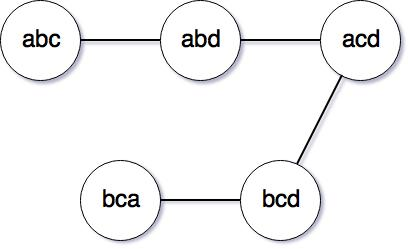
\includegraphics[scale=0.4]{alphabet}
  \end{figure}
  \newline Above graph will be formed from the given dictionary.
  \newline Below is the algorithm for constructing the graph.
  \begin{algorithm}
    \caption{Making graph from dictionary}
    \begin{algorithmic}[1]
      \Procedure{buildGraph}{Dict D}\Comment{Takes dict. as input}
        \ForAll{words in D}\Comment{Traversing dictionary}
          \ForAll{n\_words after current word}\Comment{Comparing all words occuring after current}
            \State $flag \gets$\textsc{compare}(word, n\_word)
            \If{$flag = true$}\Comment{Adding edge to undirected graph}
              \State \textsc{addEdge}(word,n\_word)
              \State \textsc{addEdge}(n\_word,word)
            \EndIf
          \EndFor
        \EndFor
        \State \Return Graph
      \EndProcedure
    \end{algorithmic}
  \end{algorithm}
  \newpage
  \noindent Now, since the graph is constructed and we will traverse the graph to find the path with minimum number of allowed edits, in short the shortest path between the nodes $A$ and $B$ in this graph. \newline
  Since we are going from $A$ to $B$, we will pick $A$ to be our initial vertex and apply $BFS$ algorithm with source vertex as $A$ to find the shortest path to $B$ as follows
  \begin{itemize}
    \item{All vertices adjacent to $A$ will be at a distance of $1$ from $A$.}
    \item{All vertices adjacent to the neighbours of $A$ (but not $A$) will be at distance $2$ from $A$.}
    \item{Following and expanding the above path keeping track of parents of nodes will give us the shortest path.}
  \end{itemize}
  Now, there might be $2$ possibilities here, either there exists a path between $A$ and $B$ or there doesn't.
  \begin{itemize}
    \item{If there does exist a path between $A$ and $B$, then it will be found by the algorithm as we are moving to adjacent levels (neighbours) one by one.}
    \item{If there doesn't exist a path between $A$ and $B$, then the graph must have been disconnected and during traversal of component containing $A$, $B$ will never be encountered and thus we can output "Path does not exist" after component containing $A$ is traversed completely.}
  \end{itemize}
  If we apply above algorithm to the mentioned example, we will get the path $$abc, abd, acd, bcd$$
  \bold{Proof of Correctness}
  \begin{proof}
    Firstly, during constructing of undirected graph, we are comparing each node with an other node once, so it is not possible for a connection to be left out between $2$ words. \newline
    Out of the $2$ possibilities of existence of paths, I am assuming the first one because second is trivially proved as $B$ will never be encountered during traversal and thus no path exists. \newline
    In case of existence of path, we are expanding from the source vertex $A$ level by level as in the case of $BFS$, so we will reach the end of the component containing $A$ and since $B$ is part of that component, we will reach $B$ eventually. \newline
    Also, at every point we are calculating the shortest path for every node from $A$ so we will always lead to a path with shortest length when we reach $B$.
  \end{proof}
  \noindent \bold{Time Complexity}
  \begin{solution}
    First finding out the time complexity of the \bold{buildGraph} procedure, we are traversing the list word by word and then multiplying that with the number of words after that. \newline
    Also, assuming right now that complexity of \bold{compare} procedure is $k$ (depends on string size).
    \begin{align*}
      T(n,k) &= k * ((n-1) + (n-2) + (n-3) + (n-4) + \dots + 1) \\
      T(n,k) &= k * \frac{n(n-1)}{2}
    \end{align*}
    Now, finding out the time complexity of the shortest path finding algorithm, the time complexity of $BFS$ is $O(|V| + |E|)$, so the time complexity of this will also be $O(|V|+|E|)$. \newline
    \newpage
    \bold{Worst Case Time Complexity} 
    \begin{myenv}
      The worst case time complexity for the \bold{buildGraph} algorithm will be $O(cd^2)$ where $d$ is number of vertices and $c$ is the time complexity of compare statement.\newline
      The worst case time complexity for the \bold{BFS} algorithm will be $O(cd^2)$ only as the max number of edges can be $\frac{d(d-1)}{2}$ \newline
      So the worst case time complexity is $$ T(c,d) = O(cd^2)$$
    \end{myenv}
  \end{solution}
}
\newpage
\section{Problem 4 Solution}{
  In this question we are given a \bold{hashtable} of size $10$ and the hash function $h(g) = g mod 10$. The collision resolution technique is Linear Probing. \newline
  There is insertion of $6$ values in the table -> 42,23,34,52,46,33 not particularly in this order. After these insertions, table looks like this. \newline
  \begin{figure}[h]
    \centering
  \begin{tabular}{l | l} 
    0 & nothing \\
    1 & nothing \\
    2 & 42 \\
    3 & 23 \\
    4 & 34 \\
    5 & 52 \\
    6 & 46 \\
    7 & 33 \\
    8 & nothing \\
    9 & nothing
  \end{tabular}
  \end{figure}
  \newline In case of Linear Probing if there is a clash, then the element is inserted in the next free slot. \newline
  So, depending on the table generated after 6 insertions, the following must be true:
  \begin{align}
    &52 \text{ must come after } 42,23,34 \text{ as } 52 \text{ clashes with } 2,3,4 \text{ slots} \label{eq:1} \\
    &33 \text{ must come after } 23,34,52,46 \text{ as } 33 \text{ clashed with } 3,4,5,6 \text{ slots}
  \end{align}
  Using eq (4.1) and (4.2), we get that $$33 \text{ will be inserted at last and } 52 \text{ will be inserted at } 4^{th} \text{ or } 5^{th} \text{time.}$$
  So, there can be $2$ possible ways to insert $52$ ($46$ may be inserted before or after $52$) and there is only $1$ way to insert $33$.\newline
  If we insert $52$ at the $4^{th}$ time, then the $3$ numbers before this must be $\{42,23,34\}$ in any order which gives us $3!$ ways. \newline
  If we insert $52$ at the $5^{th}$ time, then the $4$ numbers before this must be $\{42,23,34,46\}$ in any order which gives us $4!$ ways. \newline
  Thus, total number of ways these $6$ integers can be inserted one after the other into the hash table are $$ 3!+4! = 30$$
}
\newpage
\section{Problem 5 Solution}{
  We are given the following graph and I have to find the a \bold{DFS spanning tree} with \bold{maximum possible height}.
  \newline Choosing \bold{a} as the root vertex, applying DFS, we get the following \bold{DFS tree} and \bold{spanning tree by DFS}.
  \begin{figure}[h]
    \centering
    \begin{minipage}[h]{0.6\textwidth}
      \caption{Graph}
      \begin{minipage}[h]{0.5\paperheight}
        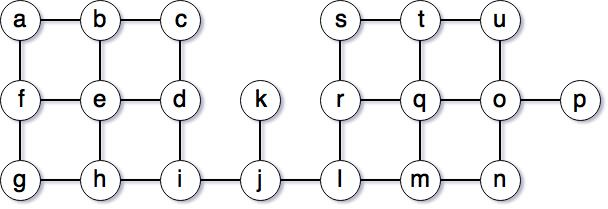
\includegraphics[width=0.6\textwidth]{graph}
      \end{minipage}
      \caption{Spanning Tree by DFS}
      \begin{minipage}[h]{0.5\paperheight}
        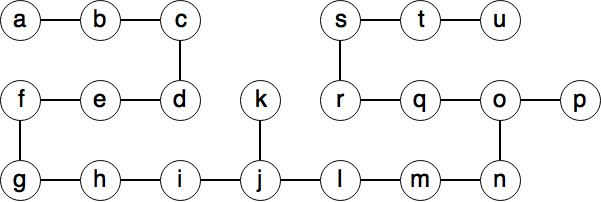
\includegraphics[width=0.6\textwidth]{DFS_spanning_tree}
      \end{minipage}
    \end{minipage}
    \hfill
    \begin{minipage}[h]{0.2\textwidth}
      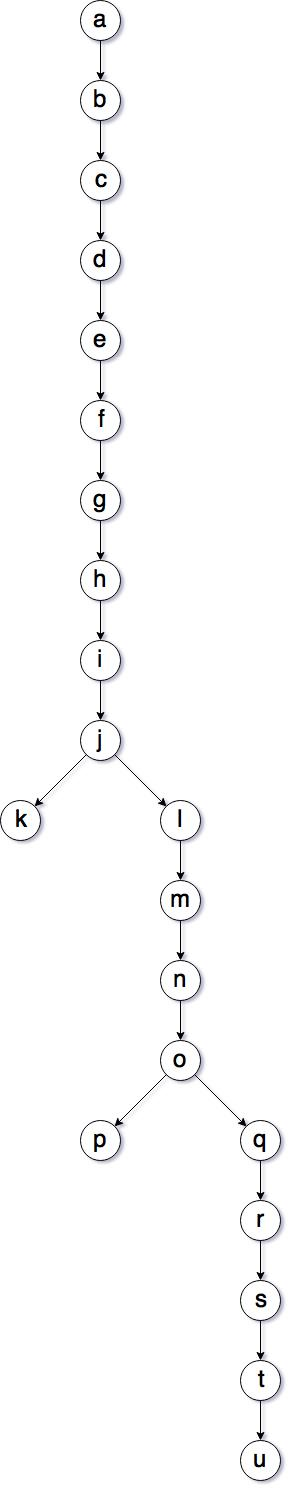
\includegraphics[width=\textwidth]{spanning_tree}
      \caption{DFS tree}
      \label{fig:spantree}
    \end{minipage}
 \end{figure}
 \newpage
 \noindent In DFS, when moving from one node to another, there is possibility of moving on any of the unvisited node.
 \newline If all of the node's neighbours have been visited then you move back to the node you came from, till you find a new node to visit. You keep on doing this procedure till all the nodes have been visited once and note the order of the traversal.
 \newline The different traversal paths while applying DFS algorithm, will get you many spanning trees out of which I have to report the spanning tree with the maximum height.
 \newline Since the number of nodes in this graph is $21$, the maximum height $H \leq 21$.
 \newline While traversing we can notice that the nodes $k$ and $p$ are $1$ degree nodes and thus they will form the leaves in the maximum height DFS tree, also they are connected to a node which is part of a cycle so they will branch out.
 \newline Thus, the maximum height $H \leq (21-2)$ and from the DFS tree figure on page \pageref{fig:spantree} we can see that the maximum height of the tree is $19$.
}
\newpage
\section{Problem 6 Solution}{
  The problem consists of a set of islands and each island is connected to one or more islands via bridges. 
  \newline Each bridge has a token associated with it which is used for crossing that bridge and each token is unique. Also there are a total of $n$ bridges.
  \newline John (our person of interest) has been given $n$ tokens ($1$ for each of the $n$ bridges) and his desire is to cross all the bridges exactly once for which he needs to know which path to travel.
  \newline \newline This problem can be considered as a graph problem where the islands are vertices and the bridges are edges and they form a connected graph.
  \newline The problem is to find a path in the graph such that we traverse all the edges exactly once.
  \newline If the graph contains a \bold{Eulerian path} or a \bold{Eulerian cycle} then that path or cycle will be the corresponding path which John needs to traverse to win, if there is no \bold{Eulerian path} or \bold{Eulerian cycle} in the graph, then John can't win.
  \newline Here is the \href{https://en.wikipedia.org/wiki/Eulerian\_path}{Source} for the proof of the above analogy and claim.
  \newline \newline As per the source, for a graph to contain a \bold{Eulerian path}, the number of odd degree vertices must be $0$ or $2$.
  \newline First we will check the above condition and if the above condition is not satisfied then John can't win as an Eulerian Path does not exist.
  \newline In an undirected graph, it is not possible to have only $1$ node with odd degree, so we will use following algorithm to check if graph is \bold{Eulerian} or not. \newline

  \begin{algorithm}
    \caption{Eulerian Graph or Not}\label{eulerian}
    \begin{algorithmic}[1]
      \Procedure{isEulerian}{Graph g}\Comment{returns true or false}
        \State $count \gets 0$
        \ForAll{$v \in  g$}\Comment{Here $v$ are vertices of graph}
          \If{deg[v] is odd}\Comment{deg[v] gives the degree of $v$}
            \State $count++$
          \EndIf
        \EndFor
        \If{$count > 2$}
          \State \Return false
        \EndIf
        \State \Return true
     \EndProcedure
    \end{algorithmic}
  \end{algorithm}

  If the above procedure returns \bold{false}, then John can't win but if it returns \bold{true}, then John can win and we can use the following algorithm to find the path which he sould follow.
  \newline \newline We will have to choose an initial vertex to begin with, i.e. the vertex from where we start traversing.
  \newline If there are $2$ vertices with odd degree then initial vertex will be one of them, otherwise any vertex can be chosen.
  \newpage
  \noindent Now, while degree of any vertex is non-zero (i.e. Edges exist in graph), follow the following steps.
  \begin{itemize}
    \item{Move to a neighbouring vertex having max degree.}
    \item{Note the Traversed edge.}
    \item{Remove the traversed edge and reduce the degrees of its ends by $1$ each.}
  \end{itemize}
  Consider the following example
  \begin{figure}[h]
    \centering
    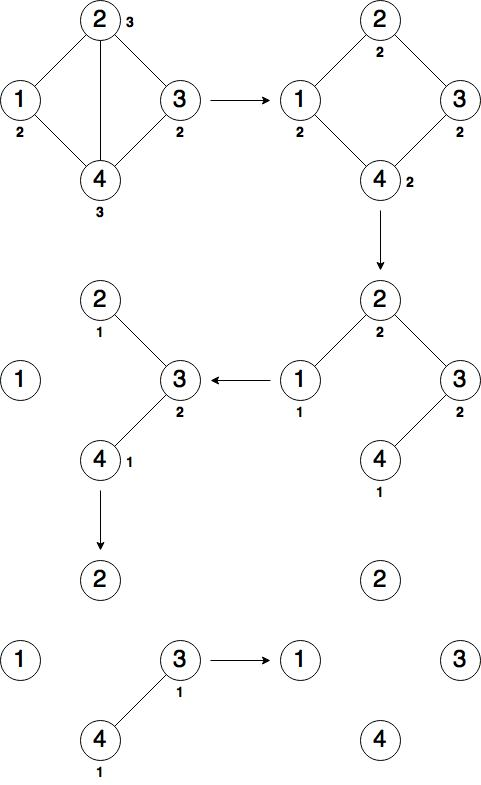
\includegraphics[scale=0.5]{euler}
  \end{figure}
  \newline The \bold{Eulerian Path} for the above example will be $$(2,4)\quad(4,1)\quad(1,2)\quad(2,3)\quad(3,4)$$
  \newpage
  \noindent The algorithm for finding the \bold{Eulerian Path} is
  \begin{algorithm}
    \caption{Eulerian Path}
    \begin{algorithmic}[1]
      \Procedure{eulerianPath}{Graph g}\Comment{Prints the Eulerian path (order of edges)}
        \State $a_v \gets $ initial vertex\Comment{Depending on $0$ or $2$ odd degree vertices}
        \While{$\exists v\text{ such that } deg[v] \neq 0$}\Comment{As long as there are edges}
          \State $deg[a_v] \gets deg[a_v] - 1$
          \State $b_v \gets adj[a_v]$\Comment{$b_v$ is the adjacent vertex with max degree}
          \State $deg[b_v] \gets deg[b_v] - 1$
          \State \bold{print } $(a_v,b_v)$
          \State $del(E(a_v,b_v))$\Comment{Removing traversed edge}
          \State $a_v \gets b_v$
        \EndWhile
      \EndProcedure
    \end{algorithmic}
  \end{algorithm}
  \newline \bold{Proof of Correctness}
  \begin{proof}
    According to algorithm, we are choosing the next vertex to be the vertex with max degree which means the vertex with degree $1$ will be chosen when we have no other choice left. \newline
    Also there can't be a situation where we have to choose between $2$ vertices such that both have degree $1$ as it is only possible when either graph is \bold{not Eulerian} or we didn't start with a vertex of odd degree even when the graph had initially. \newline
    So, at every point we will have a vertex with degree greater than $1$ to go to unless we reach the last edge, at which point we traverse the last edge and we have been to each and every edge as all the other vertices have degree $0$ (at which point while loop terminates).
  \end{proof}
  \noindent\bold{Time Complexity} \newline
  The time complexity for the above algorithm will be $O((V+E)^2)$ or $O(E^2)$ which can broken down to $O((V+E)*(V+E))$ where $(V+E)$ is the time taken by \bold{DFS} on adjacency list and it is done $2$ times to find which node to move to next time.
\end{document}
